\section{Literature Review}
\label{sec:Lit}
%Start my added work
\par Section II reviews the research methodologies used in six peer-reviewed journal articles \cite{munoz2026riskmetrics}–\cite{kobayashi2023cardinalitydro}. Non-academic and institutional sources are used only for contextual background and are excluded from the methodological comparison.
\begin{figure*}[!t]
  \centering
  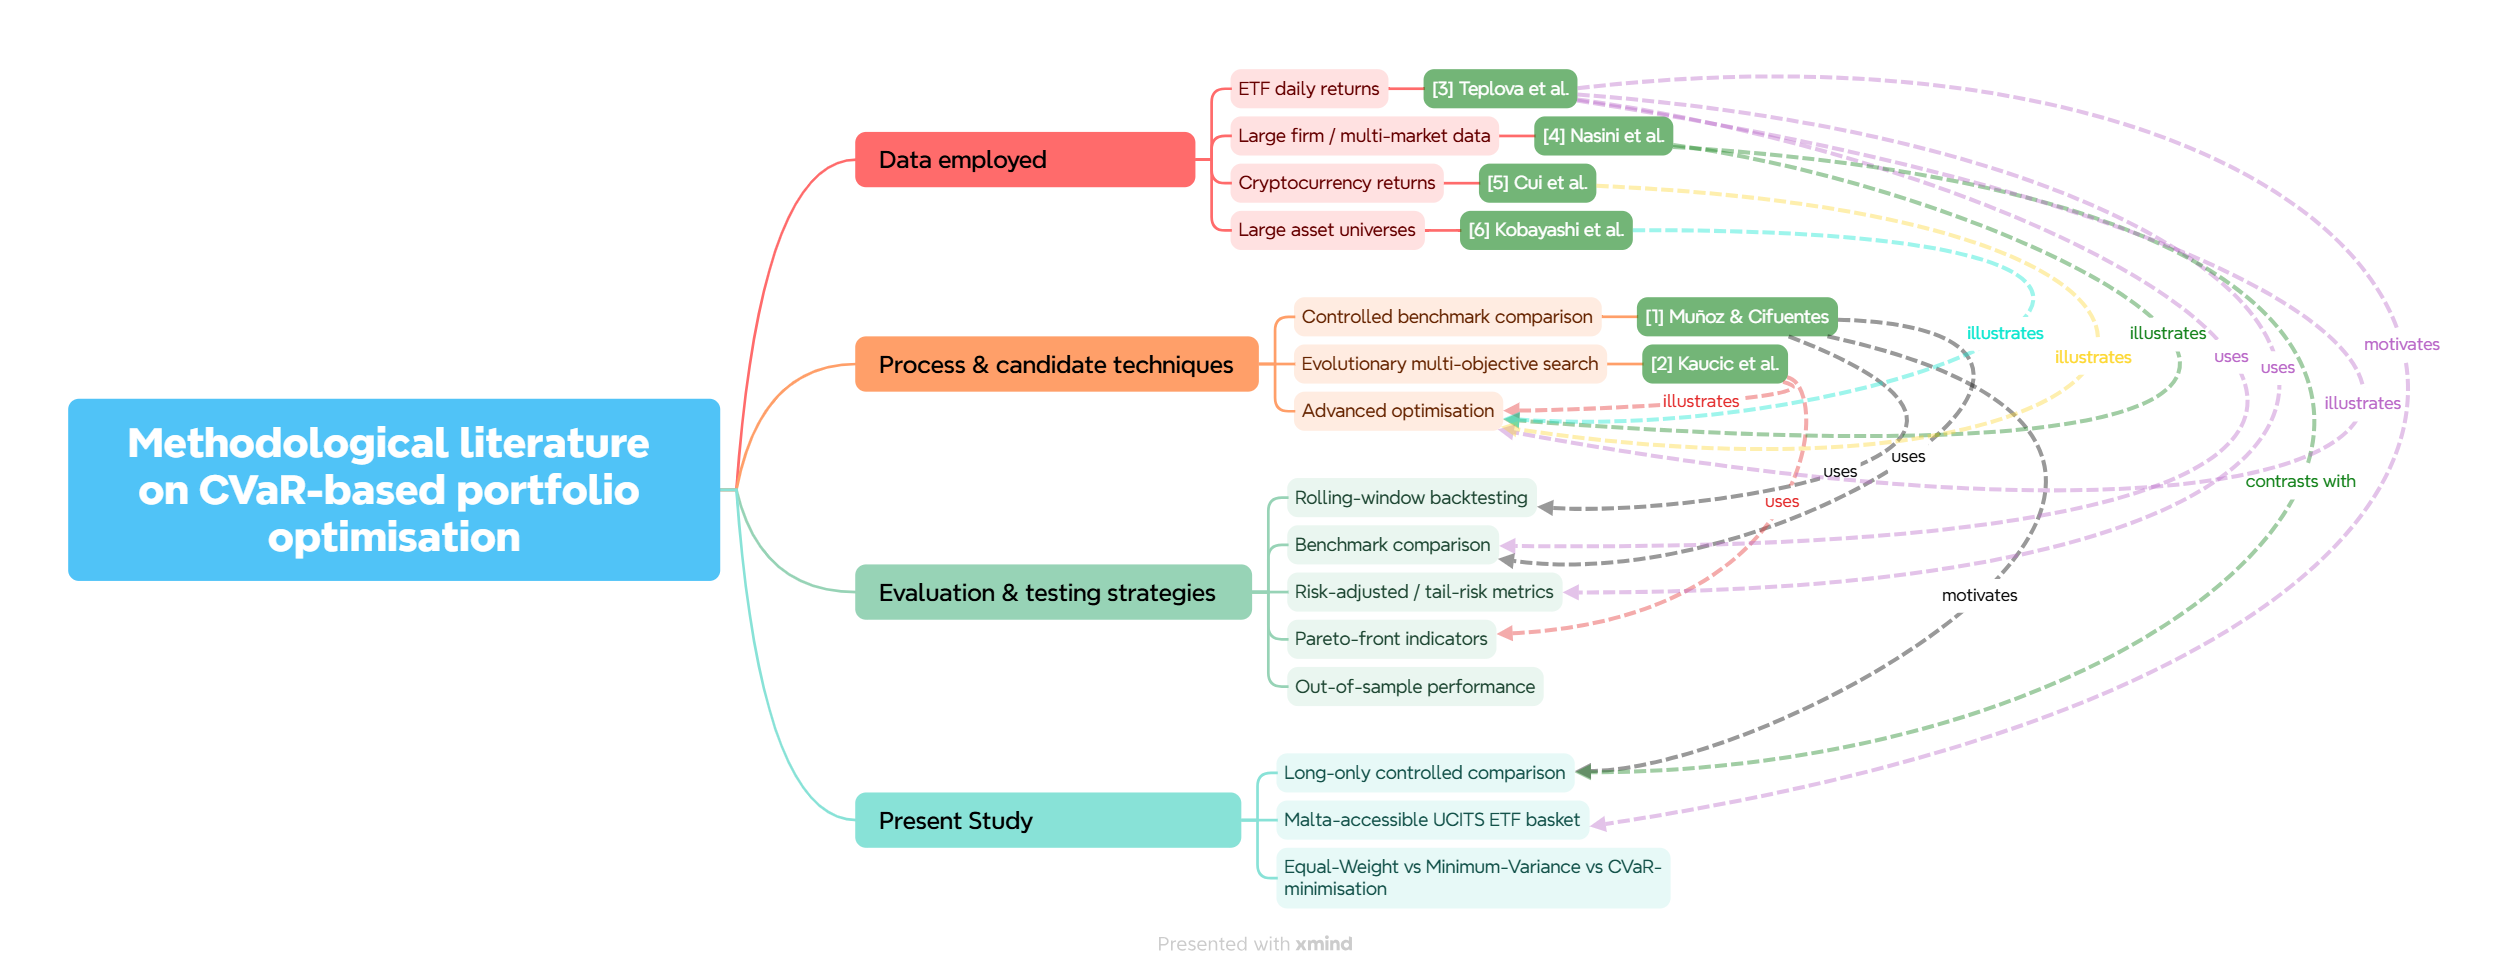
\includegraphics[width=\textwidth]{includes/litmap.png}
  \caption{Methodological literature map for CVaR-based portfolio optimisation.}
  \label{fig:lit-map}
\end{figure*}  

% \FloatBarrier
\par \hyperref[fig:lit-map]{Fig.~\ref*{fig:lit-map}} organises the reviewed methodological literature into data employed, process and candidate techniques, and evaluation and testing strategies. The map shows that prior studies mainly rely on secondary financial data and backtesting-based evaluation, but differ substantially in portfolio-construction complexity. The final branch highlights the gap addressed by the present study, namely a simpler and more transparent comparison of Equal-Weight, Minimum-Variance, and CVaR-minimisation strategies in a Malta-accessible UCITS ETF setting under identical long-only conditions.

\subsection{Overview of reviewed methodologies}
\label{subsec:lit-overview}
\par A consistent methodological pattern across the reviewed studies is the use of a positivist, quantitative design based on secondary financial data. Rather than using interviews or surveys, the reviewed papers typically rely on historical price or return series and assess portfolio-construction rules through computational testing. This broad methodological direction aligns closely with the present study, which also examines objectively measurable portfolio outcomes under controlled backtesting conditions. Accordingly, the literature map for the present study is organised around data, process, and evaluation, as illustrated in \hyperref[fig:lit-map]{Fig.~\ref*{fig:lit-map}}. 

\subsection{Data employed in prior studies}
\label{subsec:lit-data}
\par The reviewed literature shows that portfolio-optimisation research commonly uses historical market data covering several years so that both normal and stressed market conditions are represented. Muñoz and Cifuentes \cite{munoz2026riskmetrics}, for example, analyse historical returns from 2004 to 2023 and deliberately include major crisis periods to test the stability of mean-variance and CVaR formulations. Their use of rolling windows is methodologically valuable because it allows repeated comparison across time rather than relying on a single in-sample period.
\par Teplova et al. \cite{teplova2023blcopula} also use a long historical dataset, drawing on daily returns from international ETFs between 2012 and 2022. This is particularly relevant because ETFs are also the asset class used in the present study. Their data design supports realistic comparison between portfolio rules while also enabling out-of-sample testing.
\par By contrast, Nasini et al. \cite{nasini2022multimarket} use a much larger firm-level dataset across thousands of U.S. listed companies, while Cui et al. \cite{cui2023cvarrlcrypto} focus on cryptocurrency returns. Kobayashi et al. \cite{kobayashi2023cardinalitydro} also work with large asset universes in a robust optimisation setting. These studies show that broader datasets are possible, but they also increase modelling and computational complexity. For the current research, a Malta-accessible UCITS ETF basket is more appropriate because it remains sufficiently diversified while preserving transparency, feasibility, and direct relevance to the stated research context.
\par Overall, the literature suggests that the most suitable data strategy for the present study is a secondary dataset of historical ETF prices and returns, covering a sufficiently long period to include both calm and turbulent market conditions, while keeping the investable universe constant across all tested strategies.

\subsection{Portfolio-construction process and candidate techniques}
\label{subsec:lit-process}
\par The reviewed studies show that the main methodological distinction lies in the portfolio-construction process. Some studies compare classical benchmark approaches, while others embed CVaR within more advanced optimisation frameworks.
\par Muñoz and Cifuentes \cite{munoz2026riskmetrics} provide the clearest benchmark-comparison methodology. They compare mean-variance and CVaR formulations under the same target-return structure, which isolates the effect of the risk metric itself. This is highly relevant to the present study because it demonstrates how a fair experimental comparison can be achieved when constraints and data inputs are held constant.
\par Teplova et al. \cite{teplova2023blcopula} extend the process stage through copula modelling and a Black-Litterman mean-CVaR framework. Their methodology is rigorous, but it depends on parameter calibration, investor-view modelling, and dependence-structure estimation. Kaucic et al. \cite{kaucic2019riskmeasures} instead treat the process stage as a multi-objective evolutionary search problem, comparing variants of NSGA-II and SPEA 2 under downside-risk measures such as semi-variance and CVaR. Nasini et al. \cite{nasini2022multimarket} introduce a bilevel multi-market formulation, while Kobayashi et al. \cite{kobayashi2023cardinalitydro} use distributionally robust optimisation with cardinality constraints. Cui et al. \cite{cui2023cvarrlcrypto} move further still by integrating deep reinforcement learning into a mean-CVaR framework.
\par These advanced methodologies are useful as evidence that CVaR is a mature and flexible risk measure, but they are not ideal templates for the present project. The current study is not intended to propose a highly specialised optimisation engine. Instead, it aims to compare three portfolio-construction rules under identical conditions: Equal-Weight, Minimum-Variance, and CVaR-minimisation. This choice is methodologically stronger for the present study because it prioritises interpretability, control, and reproducibility over algorithmic novelty.

\subsection{Evaluation and testing strategies}
\label{subsec:lit-evaluation}
\par The literature also shows a clear methodological pattern in the evaluation stage. Studies rarely stop at in-sample optimisation. Instead, they use out-of-sample testing and compare strategies through financial performance and risk metrics.
\par Muñoz and Cifuentes \cite{munoz2026riskmetrics} use rolling windows and assess the similarity or difference between resulting portfolios under different risk formulations. Teplova et al. \cite{teplova2023blcopula} evaluate portfolio performance against benchmark strategies and report risk-adjusted outcomes as well as tail-risk behaviour. Kobayashi et al. \cite{kobayashi2023cardinalitydro} also use out-of-sample investment performance measures, while Kaucic et al. \cite{kaucic2019riskmeasures} assess optimisation quality through Pareto-front indicators in addition to portfolio risk measures.
\par Across the reviewed studies, the most relevant evaluation measures for the present research are those that capture both return and downside risk. In particular, CAGR, volatility, Sharpe ratio, Sortino ratio, VaR, CVaR, and maximum drawdown appear suitable because they allow direct comparison between standard performance and tail-risk protection. This is important because the study hypothesis does not claim that CVaR-minimisation will maximise returns; rather, it tests whether CVaR-minimisation improves downside-risk control without materially worsening return-based outcomes.

\subsection{Comparative synthesis and methodological gap}
\label{subsec:lit-gap}
\par Taken together, the reviewed literature supports three main conclusions.First, the dominant research tradition in this area is quantitative, secondary-data, and backtesting-based. This strongly supports the philosophical and methodological position already established in Section I and illustrated in Fig. 1.
\par Second, the strongest comparative designs are those that keep the dataset, constraints, and testing framework constant while varying only the portfolio rule. This is the methodological logic most clearly visible in Muñoz and Cifuentes \cite{munoz2026riskmetrics}, and it is the one most appropriate for the present study.
\par Third, although advanced methods such as copulas, bilevel programming, evolutionary optimisation, robust optimisation, and deep reinforcement learning increase technical novelty, they also introduce greater complexity and reduce transparency. For this research a simpler controlled comparison of benchmark strategies is methodologically more appropriate.
\par Finally, across the reviewed studies, the main independent element is the portfolio-construction or optimisation method, while the dependent outcomes are portfolio performance and downside-risk measures assessed through out-of-sample testing. Common testing strategies include rolling-window backtesting, benchmark comparison, and risk-adjusted performance evaluation. However, despite this methodological maturity, limited evidence compares CVaR-minimisation, minimum-variance, and equal-weight strategies in a simple, transparent, Malta-accessible UCITS ETF setting under identical long-only backtesting conditions.
% End my added work

% \begin{enumerate}
%     \item The Accents of the British Isles (ABI-1) Speech Corpus, /cite{d2004accents}
%     \item TIMIT Acoustic-Phonetic Continuous Speech Corpus, /cite{garofalo1993darpa}
%     \item Common Voice Data Set, /cite
%     \item WSJCAM0 Corpus, /cite
%     \item The Speech Accent Archive, /cite{weinberger2011speech}
%     \item The Arctic CMU Audio Database, cite{kominek2004cmu}
%     \item VoxCeleb2, cite{chung2018voxceleb2} 
% \end{enumerate}

% \begin{table}[ht]
%     \caption{Data-set comparison. Accent: Native (N); Non-Native (NN)}
%     \label{tab:Data}
%     \centering
%     \begin{tabular}{l|l|l|l|l|l}
%         \textbf{Data set} & \textbf{Speakers} & \textbf{Utterances} & \textbf{Accents}   & \textbf{Citations} & \textbf{Type} \\\hline
%         1               & 280               & 855                 & 14                & 28              & N               \\
%         2               & 630               & 6,300               & 8                 & 1,918           & N               \\
%         3               & 50,590            & 644,120             & 16                & N/A             & N \& NN            \\
%         4 & 140 & 4,400 & 4 & 346 & N \\
%         5               & 2,140             & 2,140               & \textgreater{100} & 132             & N \& NN        \\
%         6               & 18                & 1,150               & 4                 & 458             & N \& NN               \\
%         7               & 6,000              & 1,128,246          & 6                 & 168             & N \& NN  
%     \end{tabular}
% \end{table}

% \begin{table}[ht]
%     \centering
%     \caption{State of the art results}
%     \label{tab:Com}
%     \resizebox{\columnwidth}{!}{
%         \begin{tabular}{l|l|l|l}
%             \textbf{\textbf{Study}}         & \textbf{\textbf{Data set}}    & \textbf{\textbf{Metrics}} & \textbf{\textbf{Results}}                                                                   \\ \hline
%             /cite{prathyusha2017cyberbully} & Crime Investigation Forum    & F1 Score                  & \begin{tabular}[c]{@{}l@{}}CDMS: 40.75\%\\ CDCSGF: 39.75\%\end{tabular}                     \\ \hline
%             /cite{van2018automatic}         & Corpus for English and Dutch & F1 Score                  & \begin{tabular}[c]{@{}l@{}}English: 64\%\\ Dutch: 61\%\end{tabular}                         \\ \hline
%             /cite{al2016cybercrime}         & Twitter                      & F1 Score                  & 93.6\%                                                                                      \\ \hline
%             /cite{zhong2016content}         & Instagram                    & F1 Score                  & \begin{tabular}[c]{@{}l@{}}SVM Classifier: 95.00\%\\ Image Classifier: 68.08\%\end{tabular} \\ \hline
%             /cite{reynolds2011using}        & Formsrping                   & Accuracy                  & 78.5\%                                                                                      \\ \hline
%             /cite{dinakar2011modeling}      & Youtube                      & Accuracy                  & 66.70\%        \\   \hline        
%         \end{tabular}
%     }
% \end{table}

% \par The final recommended part in a good literature review is a review in the evaluation metrics used. It is not possible to cover all possible evaluation metrics but in most cases there is a classification problem, which would require something called a confusion matrix. Consider the problem of recognising and distinguishing an image of a cat from that of a dog. You will have a data set split into training and testing. Both will have the ground truth, what the image is actually showing. This ground truth, in the case of the training data set will be used for the creation of the Artificial Intelligence (AI) model, whilst the ground truth in the testing data set will be used to compare the predicted classification. The predictions are plotted in a confusion matrix as shown in Table~\ref{tab:CatDog}. The same table can be extended to have more than 2 categories such as introducing the mouse category. Then you need to cycle the focus for each category as shown in Table~\ref{tab:CatObjective} and Table~\ref{tab:DogObjective}, then extract the key values namely:
% \begin{enumerate}
%     \item \textbf{True Positives (TP)} - This refers to the correctly predicted positive values i.e. the value of both the actual class and predicted class is yes. 
%     \item \textbf{True Negatives (TN)} - These are the correctly predicted negative values i.e. the value of both actual class and predicted class is no.
%     \item \textbf{False Positives (FP)} - It indicates values where the actual class is no but the predicted class is yes.
%     \item \textbf{False Negatives (FN)} - It indicates values where the actual class is yes but the predicted class in no.
% \end{enumerate}

% \begin{table}
%     \caption{Sample Cat vs Dog Confusion Matrix}
%     \label{tab:CatDog}
%     \centering
%     \begin{tabular}{ll|ll}
%     ~      & ~   & \textbf{Predicted} & ~   \\
%     ~      & ~   & Cat       & Dog \\ \hline
%     \textbf{Actual} & Cat & 33        & 2   \\
%     ~      & Dog & 5         & 30  \\
%     \end{tabular}
% \end{table}

% \begin{table}
%     \caption{Cat category evaluation metrics}
%     \label{tab:CatObjective}
%     \centering
%     \begin{tabular}{ll|ll}
%     ~      & ~   & \textbf{Predicted} & ~   \\
%     ~      & ~   & Cat       & Not-Cat \\ \hline
%     \textbf{Actual} & Cat & TP        & FN   \\
%     ~      & Not-Cat & FP         & TN  \\
%     \end{tabular}
% \end{table}

% \begin{table}
%     \caption{Dog category evaluation metrics}
%     \label{tab:DogObjective}
%     \centering
%     \begin{tabular}{ll|ll}
%     ~      & ~   & \textbf{Predicted} & ~   \\
%     ~      & ~   & Not-Dog       & Dog \\ \hline
%     \textbf{Actual} & Not-Dog & TN        & FP   \\
%     ~      & Dog & FN         & TP  \\
%     \end{tabular}
% \end{table}

% \par The confusion matrices are used to provide evaluation metrics such as Accuracy, Precision, Recall and F1-Score. Depending on the subject matter being researched the proper metrics need to be quoted, thus the need to research this in academic literature. For a quick but reliable reference you can consider Wikipedia's dedicated page\footnote{\url{https://en.wikipedia.org/wiki/Confusion_matrix}}.

% \begin{enumerate}
%     \item \textbf{Accuracy (ACC)} - This shows the measure of effectiveness of the machine learning model.
%     \begin{equation} 
%      Accuracy (ACC)= \frac{TP + TN}{P + N}
%     \end{equation}
%     \item \textbf{Precision (PPV)} - Precision is the ratio of correctly predicted positive values to the total predicted positive values. This metric highlights the correct positive predictions out of all the positive predictions. High precision indicates low false positive rate.
%     \begin{equation} 
%      Precision (PPV)= \frac{TP}{TP + FP}
%     \end{equation}
%     \item \textbf{Recall (TPR)} - The recall is the ratio of correctly predicted positive values to the actual postive values. Recall highlights the sensitivity of the algorithm i.e. out of all the actual positives how many were caught by the program.
%     \begin{equation} 
%      Recall (TPR)= \frac{TP}{P}
%     \end{equation}
    
%     \item \textbf{F1 Score} - F1 Score is the weighted average of Precision and Recall. Therefore, this score takes both false positives and false negatives into account. Intuitively it is not as easy to understand as accuracy, but F1 is usually more useful than accuracy, especially if you have an uneven class distribution.
%     \begin{equation} 
%      F1 Score = \frac{2TP}{2TP + FP + FN}
%     \end{equation}
% \end{enumerate}
